\documentclass[]{article}
\usepackage[style=numeric,backend=biber,sorting=none]{biblatex}
\usepackage{graphicx}
\usepackage{float}
\addbibresource{references.bib}

% Title Page
\title{Financial Analysis Report}
\author{Mark Paveszka}


\begin{document}
\maketitle

\newpage

\begin{abstract}
\end{abstract}

\newpage

\tableofcontents

\newpage

\section{Introduction}
\paragraph{}
As a result of modern technology, the way things are done is very different compared how it was twenty years ago. Since then everything has been speeding up, including a key area of society, namely: education. In the past fifteen to twenty years several businesses emerged to make education better and easier for both students and teachers. These businesses usually try to create software artefacts to improve some aspect of the broader field. Such software artefacts are innovative learning tools and learning management systems (LMS). One of the most well-known companies in the education technology sector is Blackboard \cite{Blackboard_UK}. They provide several applications to improve the quality of teaching in higher education, business and governmental institutes. They are mostly known for Blackboard Learn \cite{Blackboard_Learn}, which is one of the most popular learning management systems currently available on the market based on data collected by Client Stat \cite{VLE-Data} and analysed by Edutechinca \cite{VLE-2020-IMG}. The aggregation of this data is shown in Figures \ref{fig:LMS-2020} and \ref{fig:LMS-2020-6-year} which depict the market share of the most popular learning management systems in four different regions. For the purpose of this analysis only the data regarding the UK will be considered. The main competitors to Blackboard are Moodle, Canvas and Brightspace. 

\begin{figure}
    \centering
    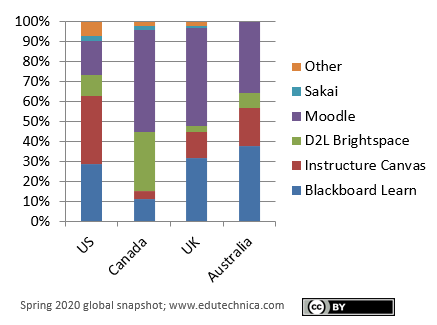
\includegraphics[width =\linewidth]{lms-vle-2020.png}
    \caption{LMS market share in 2020. \cite{VLE-2020-IMG}}
    \label{fig:LMS-2020}
\end{figure}

\begin{figure}
    \centering
    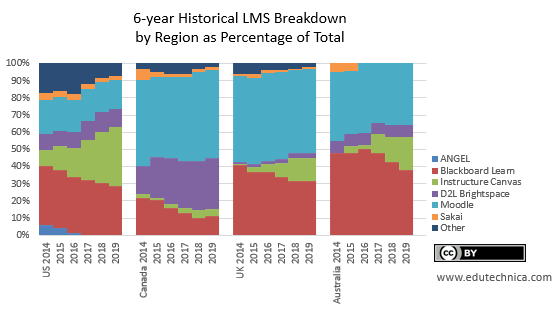
\includegraphics[width =1.2\linewidth]{lms-vle-2020-y5.png}
    \caption{6-year historical LMS data by region. \cite{VLE-2020-IMG}}
    \label{fig:LMS-2020-6-year}
\end{figure}

\paragraph{}
To obtain data some data about these companies an online tool, namely Software Advice \cite{Software-Advice} was used. This tool allowed for comparisons between the companies, which provided further insight about them. The result showed that Blackboard, Canvas and Brightspace compete in the same price range, while Moodle is cheaper to use. After examining different sources it is clear that Blackboard is not a cheap software to use \cite{Blackboard-v-Moodle}, however it provides a wide variety of features for the institutions that opt to use their system.

\paragraph{}
In 2017 the education technology sector in the UK worth around £170m \cite{Government-Strategy}. This number by 2021 is expected grow to to £3.4bn which shows that there is a lot of potential in this sector. However it is worth noting that the LMS market is part of the education technology sector and even though there will be growth it might not be that significant. Also globally there is not much change \cite{VLE-2020-IMG} in the usage of these systems compared to previous years based on Edutechnica's analysis. Globally speaking there is going to be a massive growth \cite{Markets-and-Markets} even when looking at what is projected for Europe (Figure \ref{fig:Markets-LMS}). However it is worth noting that market size of Europe will only be a small portion of the global market.

\begin{figure}
    \centering
    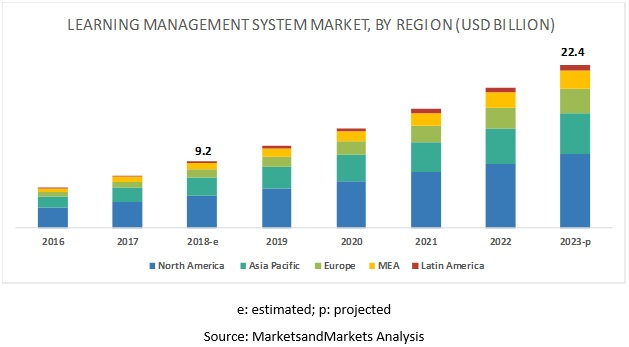
\includegraphics[width =1.2\linewidth]{learning-management-systems-market5.jpg}
    \caption{Market growth projection. \cite{Markets-and-Markets}}
    \label{fig:Markets-LMS}
\end{figure}

\newpage
\section{Financial Analysis}
\paragraph{}
In order to determine how successful Blackboard is, its financial situation needs to be examined. The following information was obtained by using FAME which is a financial database about UK based companies. To perform the analysis ratios will be used. These ratios can be found in Table \ref{tab:Ratios-BB}. In Blackboard's FAME report \cite{FAME-Blackboard} the latest data entry was created in 2018. This data suggests that for the past two years the shareholder funds were decreasing somewhat. However before that this number jumped from £860k to £65m which indicates a large scale investment into the company. In 2017 the ROCE (Return on Capital Employed) ratio dropped below 0. The -14.24\% ROCE is due to the fact that the company generated a massive loss (PBT) of £-8m. This troubling trend continued in 2018, however the situations was a bit better as the ROCE value was -1.65\% which is still not negative, however it is significantly better than the 2017 one. These issues could be explained by events that happened to the company during these years. First of all Moodle ended their partnership with Blackboard \cite{Moodle-breaks-up-with-Blackboard}, which have lowered the trust in their customers. The extent this event affected the company was quite severe as they have lost their very first customers (Cornell University) in the same year \cite{Cornell-leaves-BB}. These two events combined could have easily resulted in loss of trust from other customers. It is worth noting that throughout this period, and even today Blackboard is receiving a lot of complaints for not having user friendly graphical interfaces \cite{BB-Reviews}, which could also suggest that customers were not satisfied about its products.
%TABLE
\begin{table}
\centering
\begin{tabular}{||c | c | c | c | c||} 
\hline
Ratio & 2018 & 2017 & 2016 & 2015 \\ [0.5ex] 
\hline\hline
ROCE & 1 & 6 & 87837 & 787 \\ 
\hline
Return on shareholders' fund & 2 & 7 & 78 & 5415 \\
\hline
\end{tabular}
\caption{Ratios for Blackboard (UK) Limited from 2018 to 2015}
\label{tab:Ratios-BB}
\end{table}

\newpage

\printbibliography{}

\end{document}          
